\section{Discussion}
\label{sec:discussion}

The experimental results presented in Section~\ref{sec:results}  provided to us an overview of the performance results of evaluated methods, in terms of their effectiveness and efficiency, which are discussed in this section.

Figures~\ref{fig:non-deep-methods-efficacy-and-efficiency} and~\ref{fig:deep-methods-efficacy-and-efficiency} summarize, for non-deep and deep methods, respectively, the obtained results considering the metrics used to evaluate the effectiveness of the evaluated methods (i.e., Precision, Recall, and F-measure), along with
the metrics for measuring the efficiency of these methods, considering the ICDAR'11 and ICDAR'13 datasets. 

As we can observe in Figure~\ref{fig:non-deep-methods-efficacy-and-efficiency}, the SnoopText method presented several limitations in terms of efficiency,  although it has achieved very competitive results in terms of effectiveness.  When we take a look at the SnoopText's implementations, we can see that several improvements can be done towards minimizing the computer resources required for this method. For instance, the authors saved the pre-trained models without using any data compression. Also, the re-implementation of this method considering a faster programming language (C/C++) can potentially improve considerably the time consumption.

The Scene Text Recognition method also achieved very competitive results for the ICDAR'11 dataset, as well as impressive results concerning the processing time and disk usage, in both datasets. However, the major limitation of this method concerns the low precision achieved in the experimental results, from which we glimpse some further investigation such as the use of moderns visual descriptors in replacement of descriptors proposed in the original paper. In fact, the Canny Text Detection presented competitive results by adopting the mean LBP to build a second-stage pruning classifier.

Regarding the deep learning-based methods, we also identify several limitations in terms of effectiveness and efficiency (Fig.~\ref{fig:deep-methods-efficacy-and-efficiency}). Firstly, the most accurate networks, in terms of precision and recall, obtained the lowest results in terms of processing time (SSD-MobileNetV2) or disk usage (SSTD). On the other hand, the SqueezeDet network was the most efficient network, which obtained a very impressive result considering the processing time and disk usage. But, at the same time, this network achieved poor results, in comparison with other networks, mainly in terms of its precision. These findings suggest  that further investigation is needed towards improving the efficiency of the most accurate networks.

Finally, different from to what was pointed out by~\cite{Ye2015PAMI}, experimental results with deep learning architectures proposed for object detection problems (e.g., MobilenetV2 and YOLOv3) suggest that adapting those networks for text detection is a promising research venue. Along with these networks, the TextBoxes++ presented a good balance between effectiveness and efficiency and also it seems to be a promising method for further investigation.

% The performed comparative study allows us to point out the following considerations:
% \begin{enumerate}
%     \item Different from to what was pointed out by~\cite{Ye2015PAMI}, experimental results with deep learning architectures proposed for object detection problems (e.g., MobilenetV2 and YOLOv3) suggest that adapting those networks for text detection is a promising research venue.
% \end{enumerate}
%
\begin{figure}[H]
    \centering
    \begin{subfigure}[t]{0.98\textwidth}
        \centering
        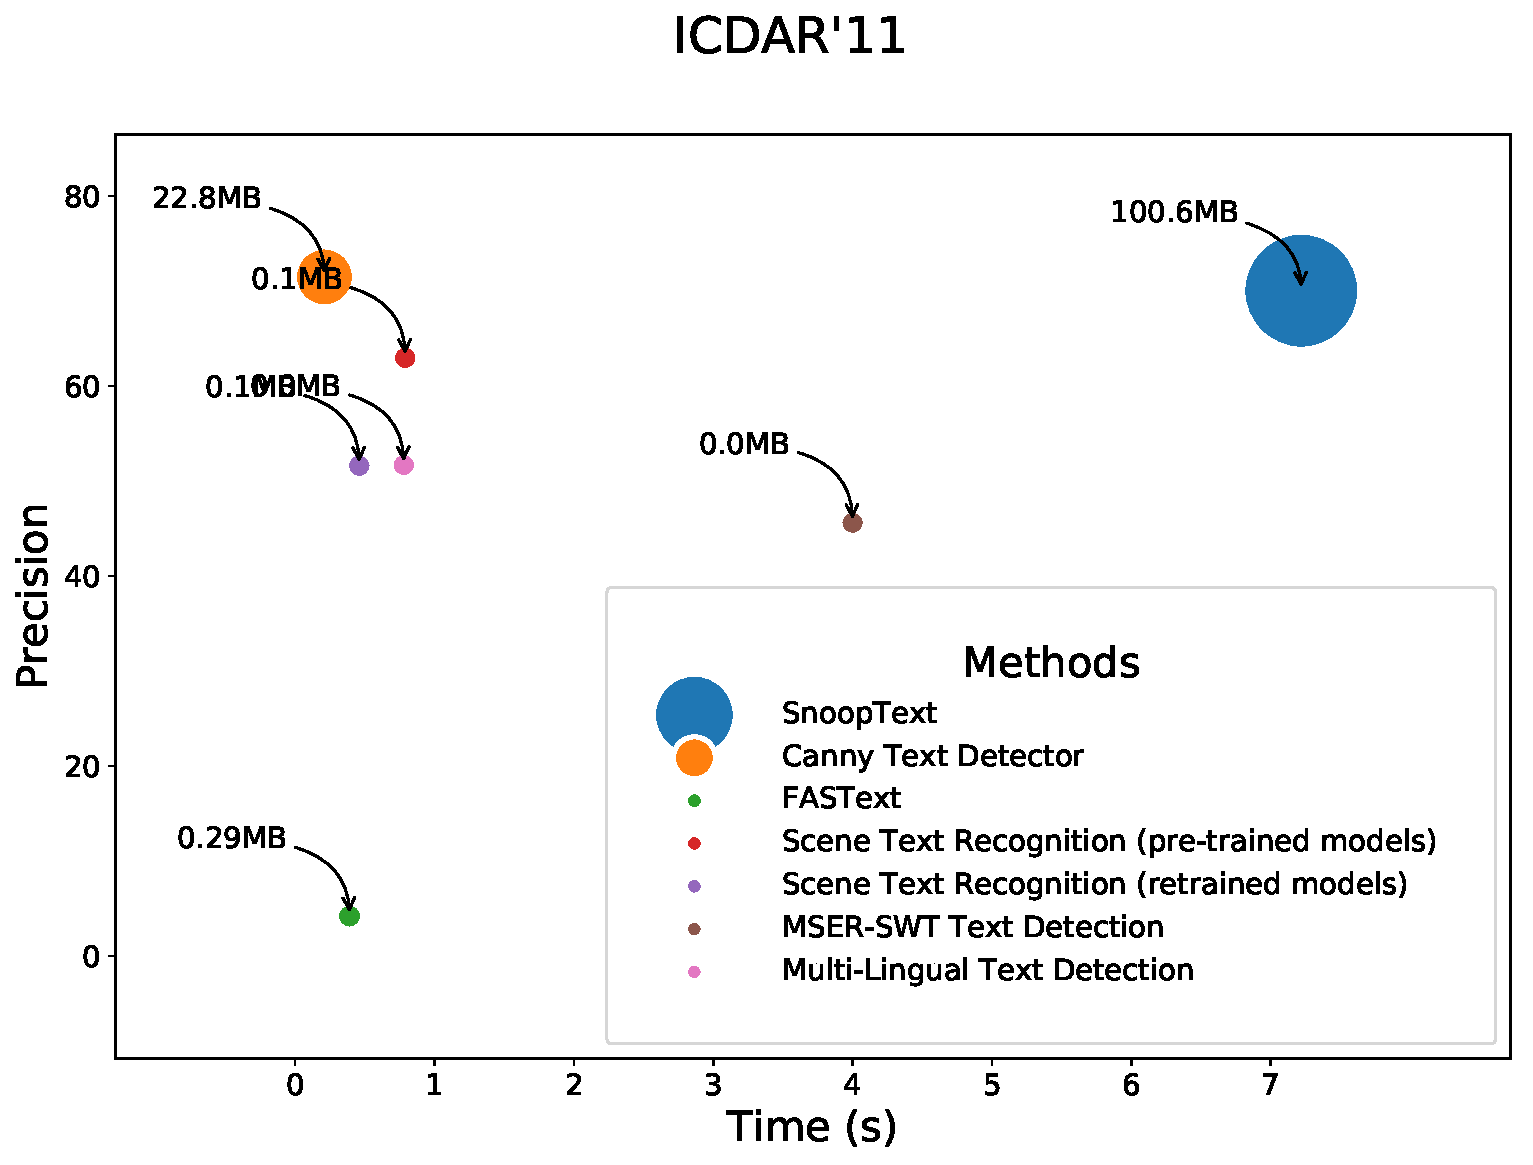
\includegraphics[height=0.25\textheight]{figs/efficacy-and-efficiency/non-deep-methods-icdar11-precision.pdf}
        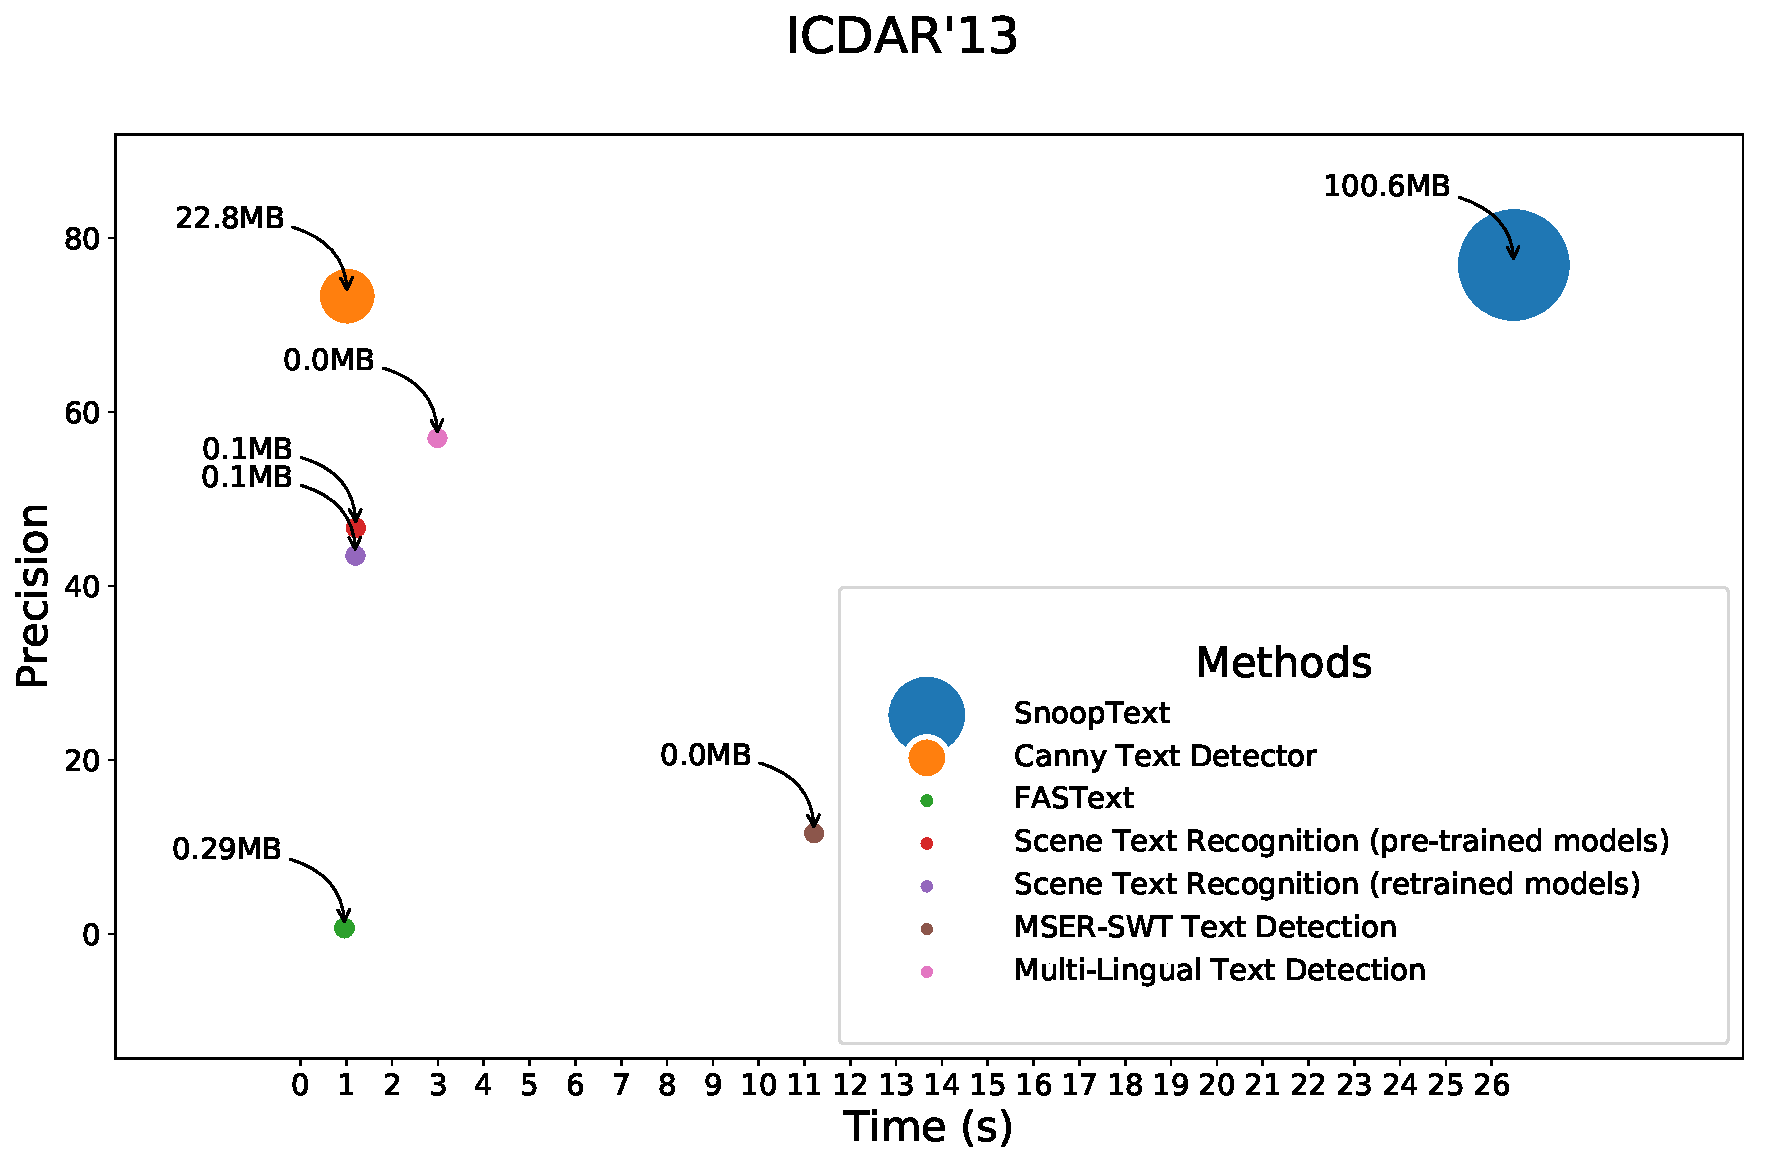
\includegraphics[height=0.25\textheight]{figs/efficacy-and-efficiency/non-deep-methods-icdar13-precision.pdf} \\
        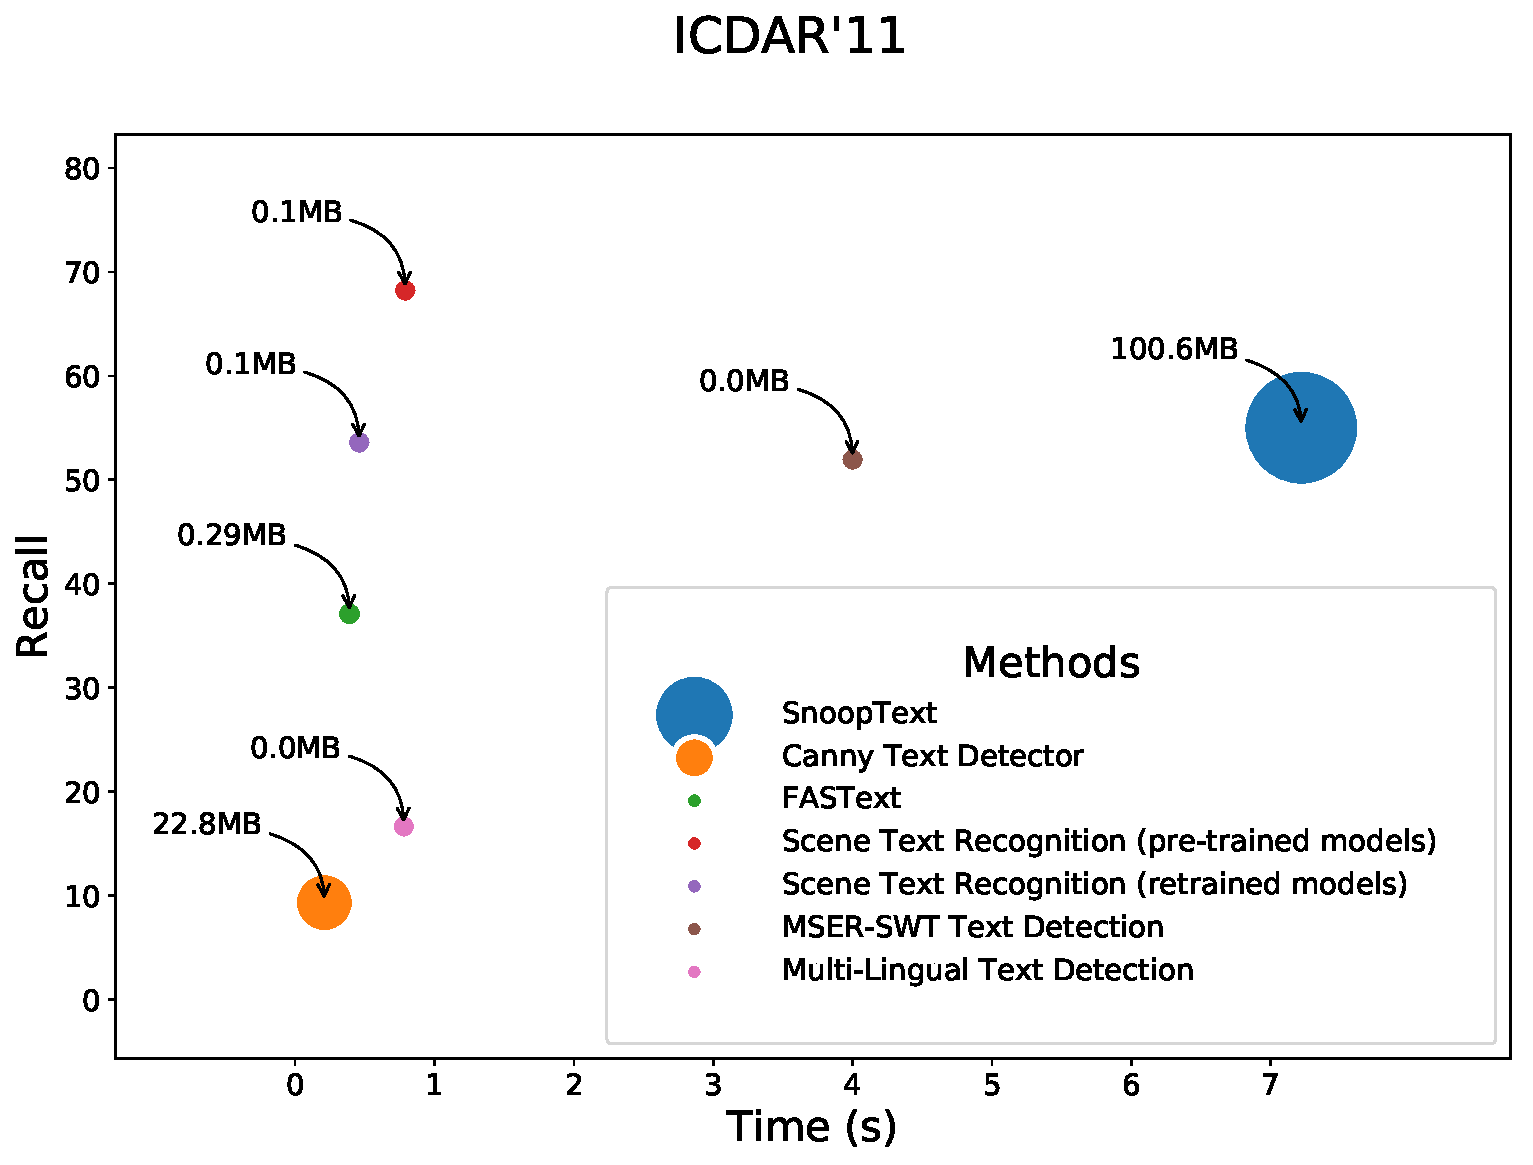
\includegraphics[height=0.25\textheight]{figs/efficacy-and-efficiency/non-deep-methods-icdar11-recall.pdf}
        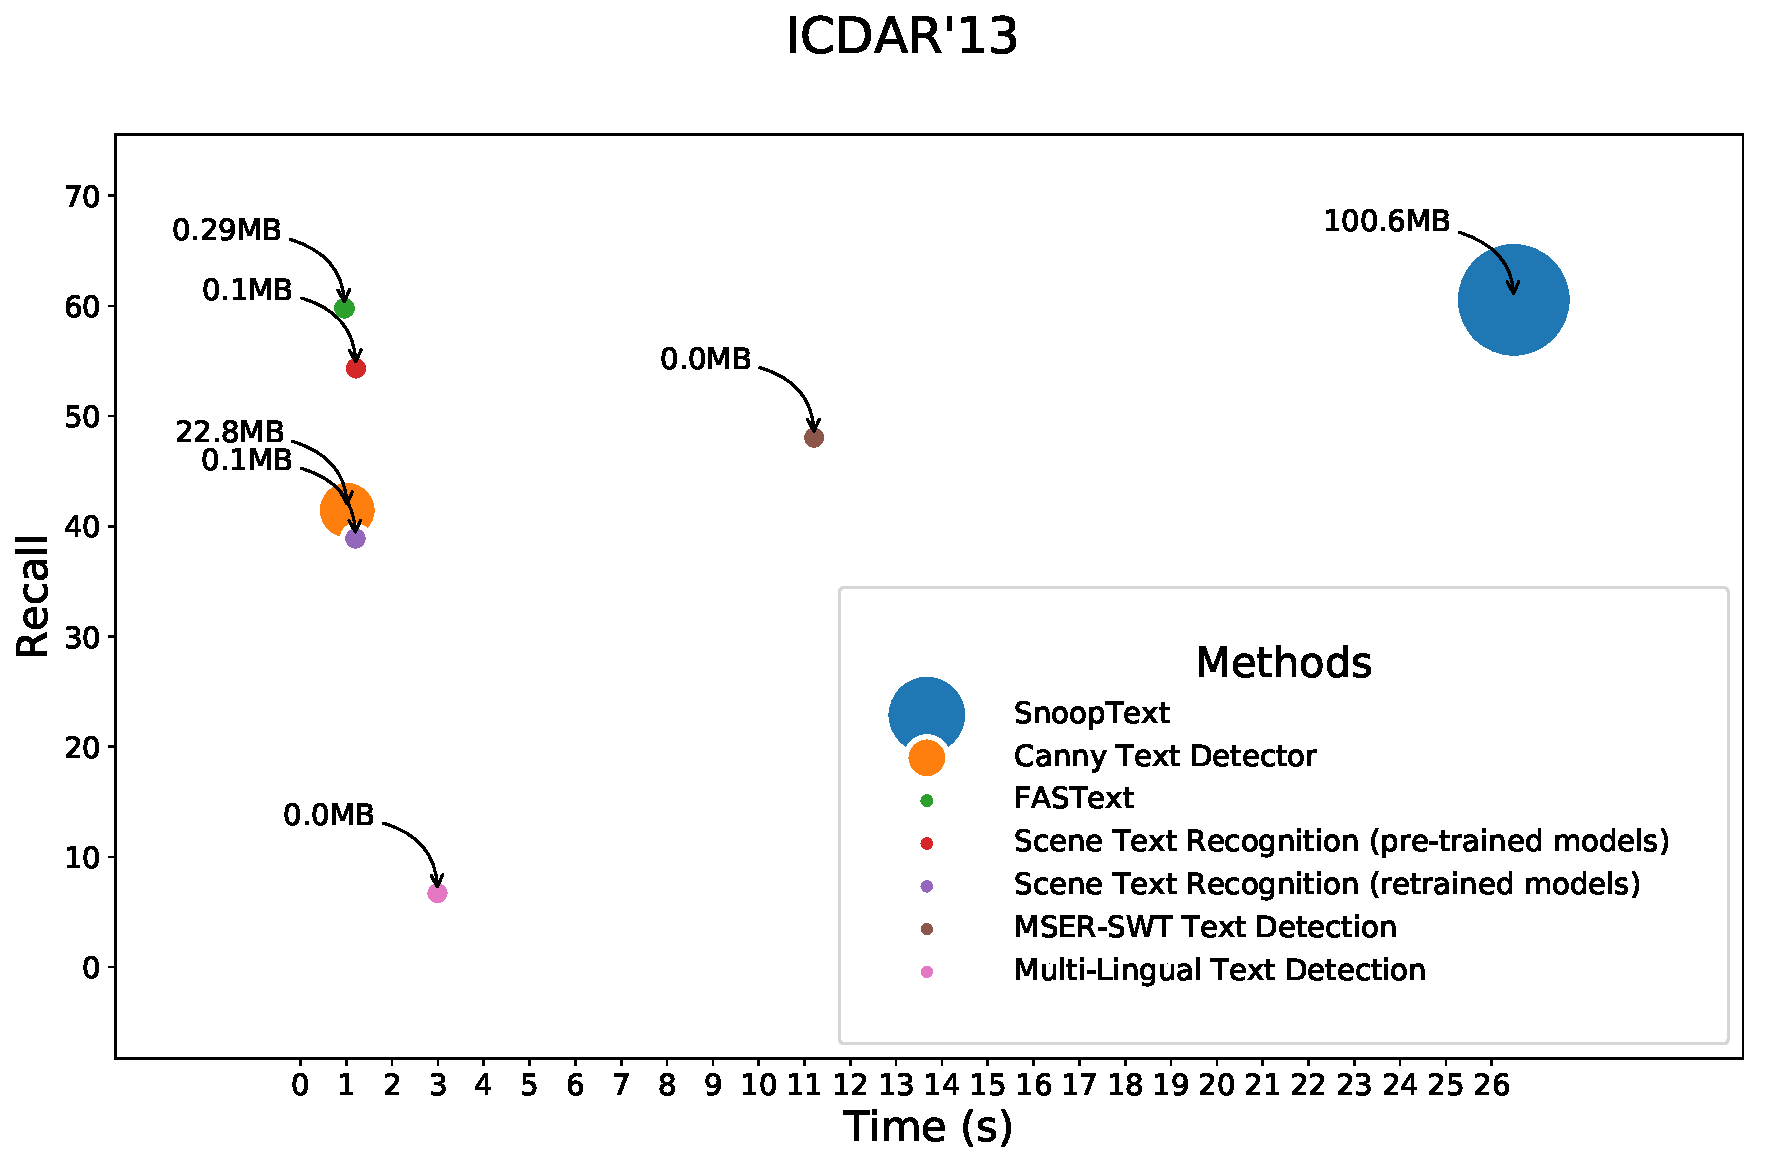
\includegraphics[height=0.25\textheight]{figs/efficacy-and-efficiency/non-deep-methods-icdar13-recall.pdf} \\
        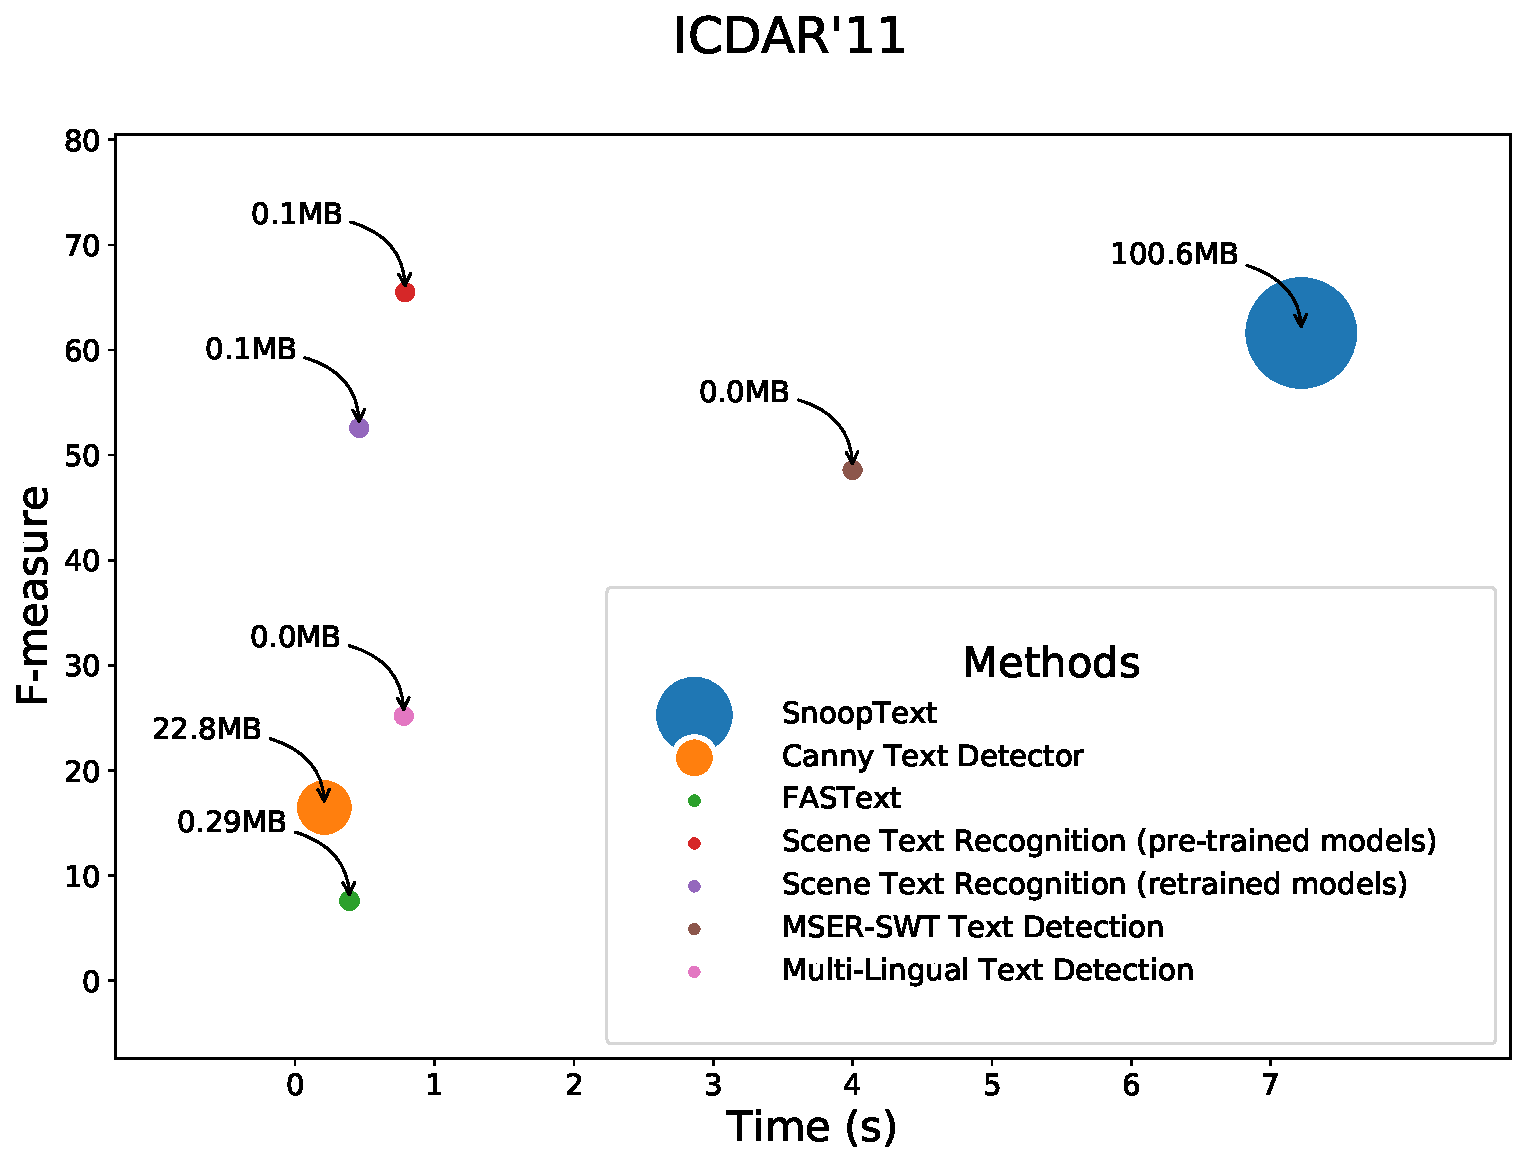
\includegraphics[height=0.25\textheight]{figs/efficacy-and-efficiency/non-deep-methods-icdar11-f-measure.pdf}
        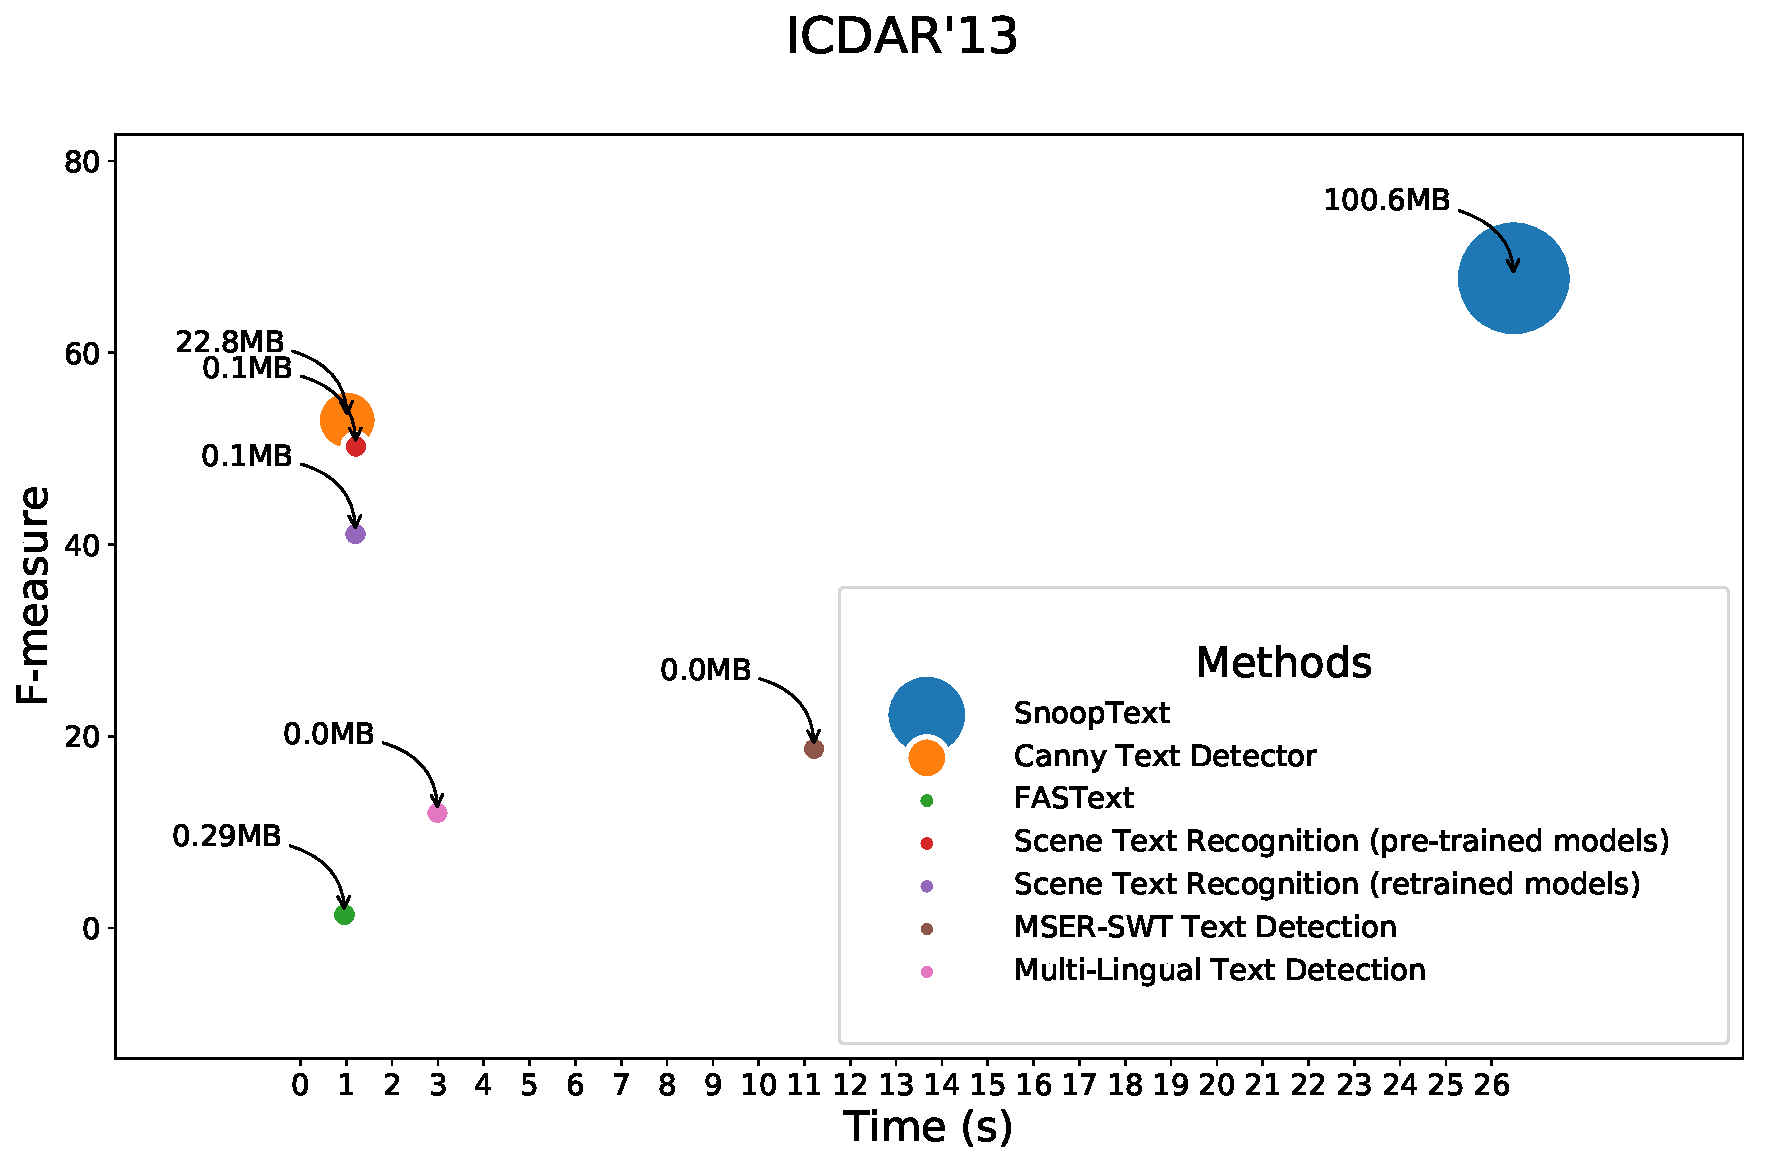
\includegraphics[height=0.25\textheight]{figs/efficacy-and-efficiency/non-deep-methods-icdar13-f-measure.pdf}
    \end{subfigure}
    \caption{Comparison results among the non-deep-based methods considering aspects of efficacy and efficiency.}
    \label{fig:non-deep-methods-efficacy-and-efficiency}
\end{figure}
%
\begin{figure}[H]
    \centering
    \begin{subfigure}[t]{0.98\textwidth}
        \centering
        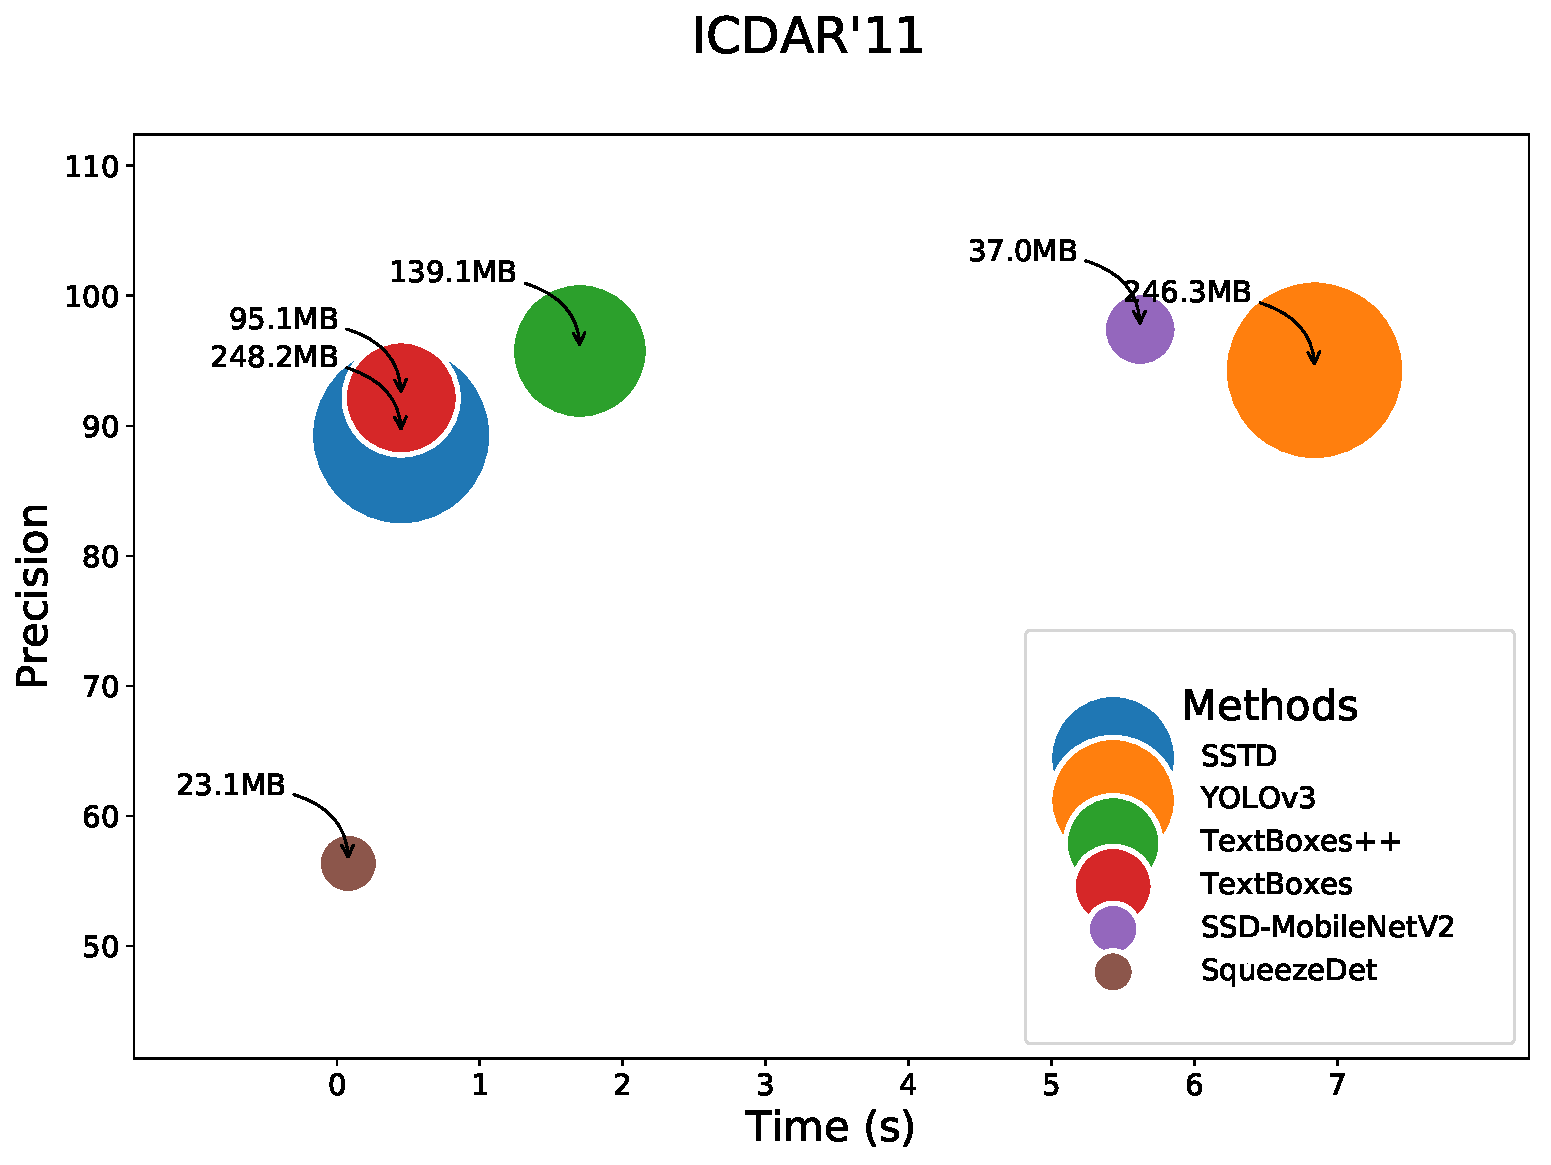
\includegraphics[height=0.25\textheight]{figs/efficacy-and-efficiency/deep-methods-icdar11-precision.pdf}
        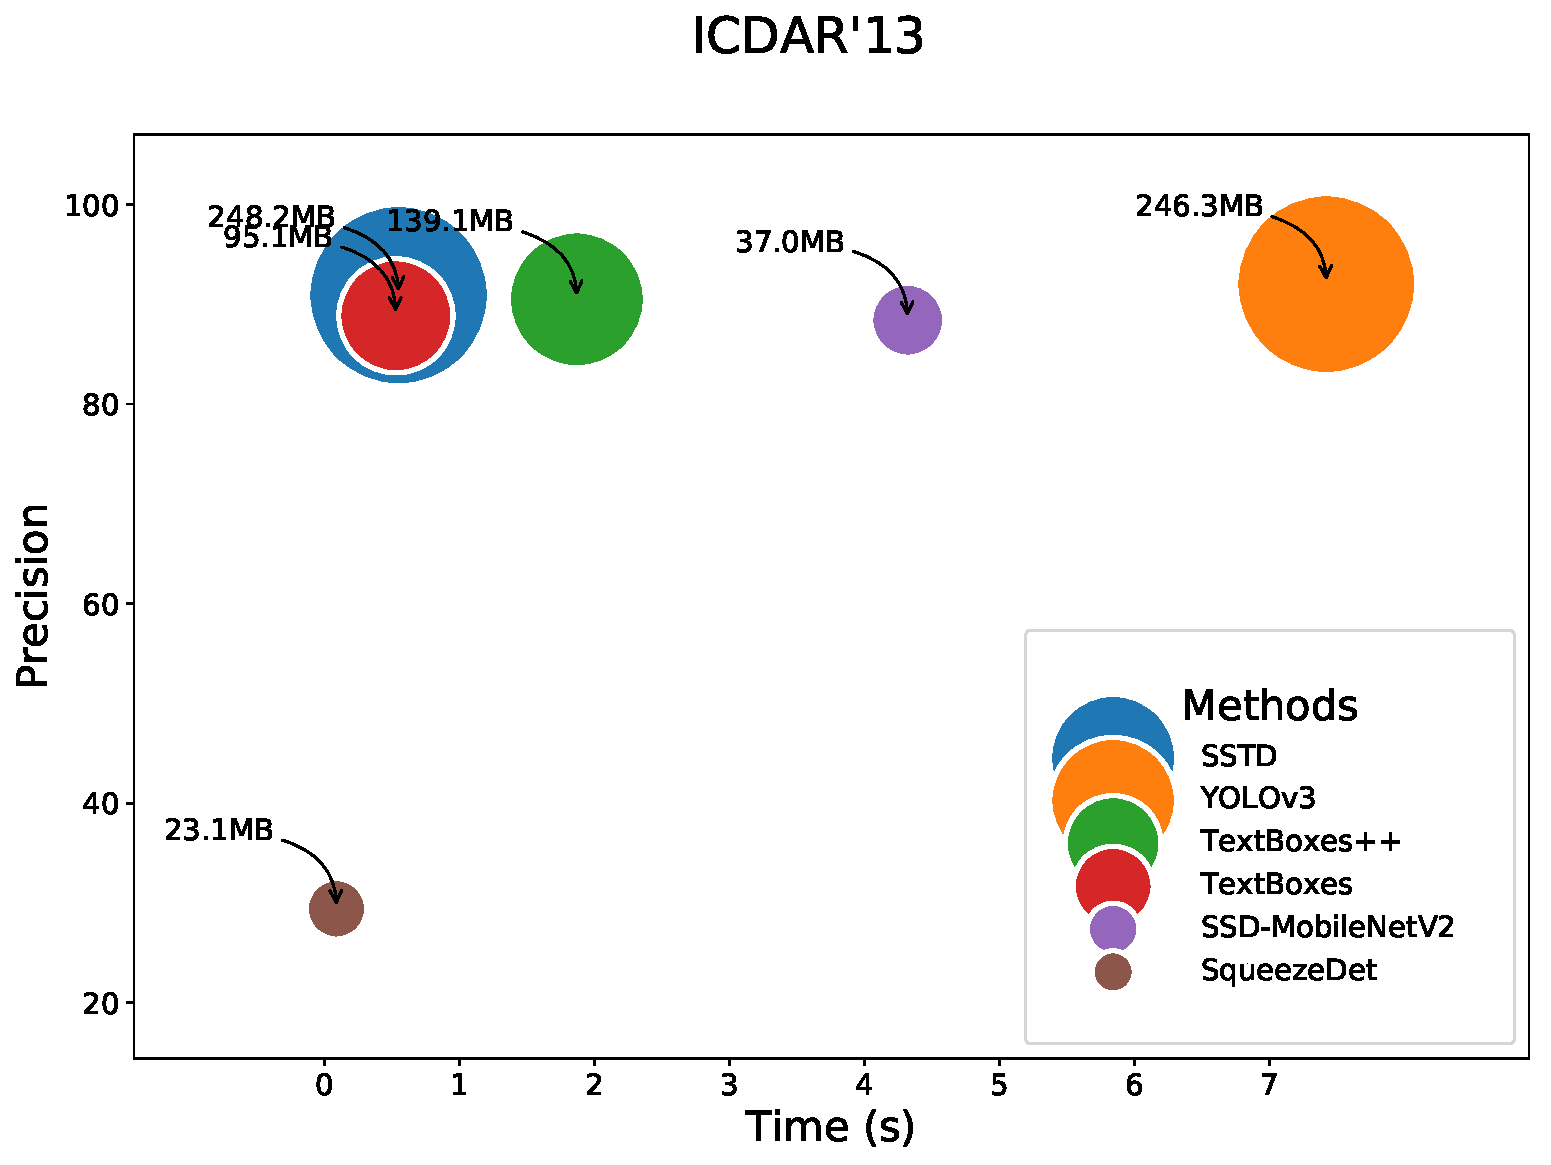
\includegraphics[height=0.25\textheight]{figs/efficacy-and-efficiency/deep-methods-icdar13-precision.pdf} \\
        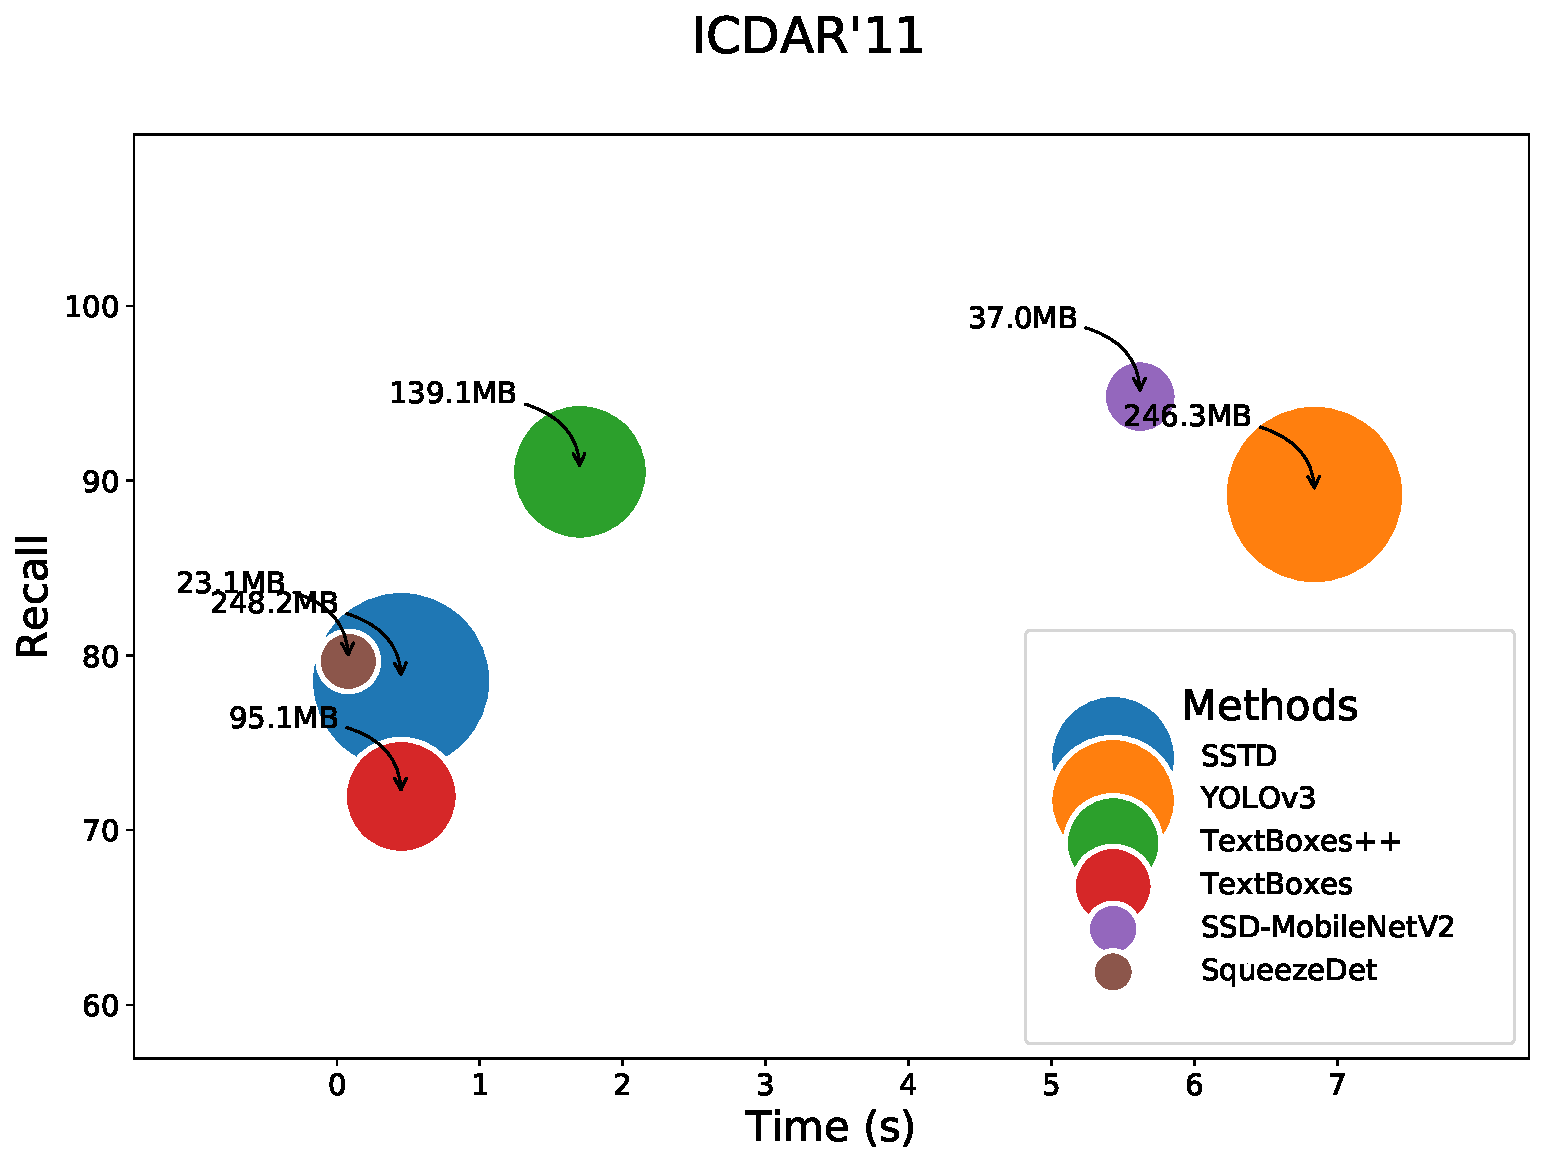
\includegraphics[height=0.25\textheight]{figs/efficacy-and-efficiency/deep-methods-icdar11-recall.pdf}
        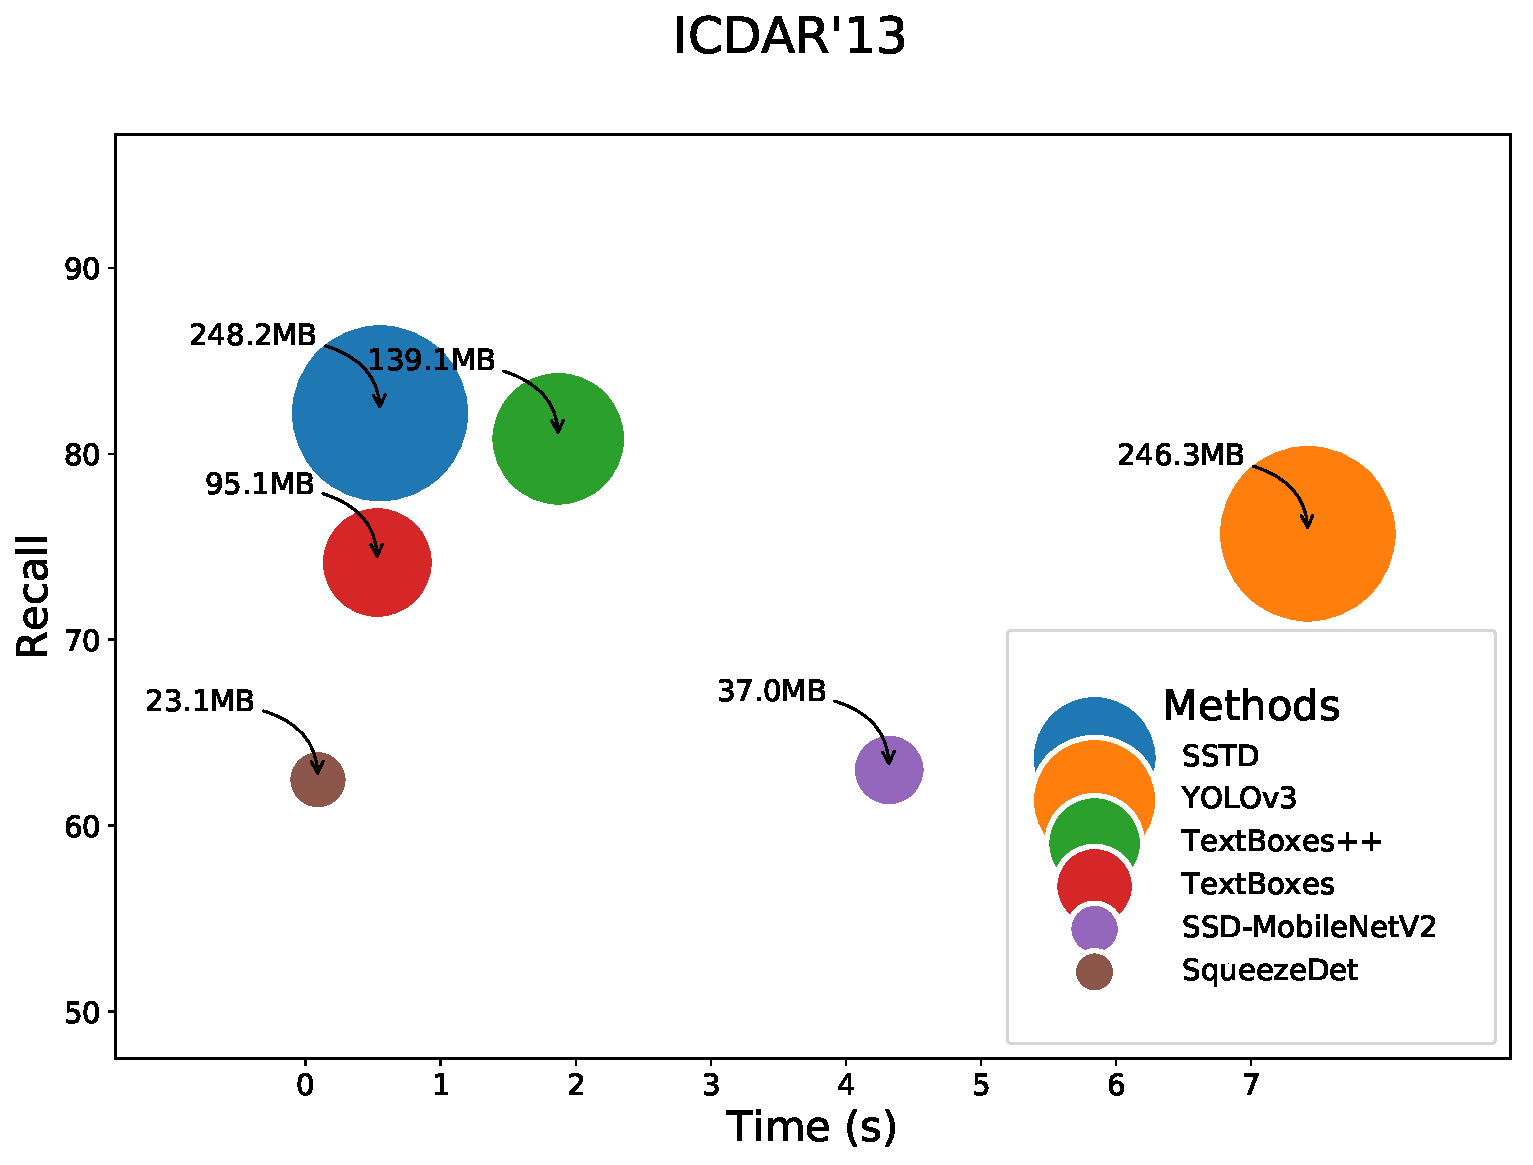
\includegraphics[height=0.25\textheight]{figs/efficacy-and-efficiency/deep-methods-icdar13-recall.pdf} \\
        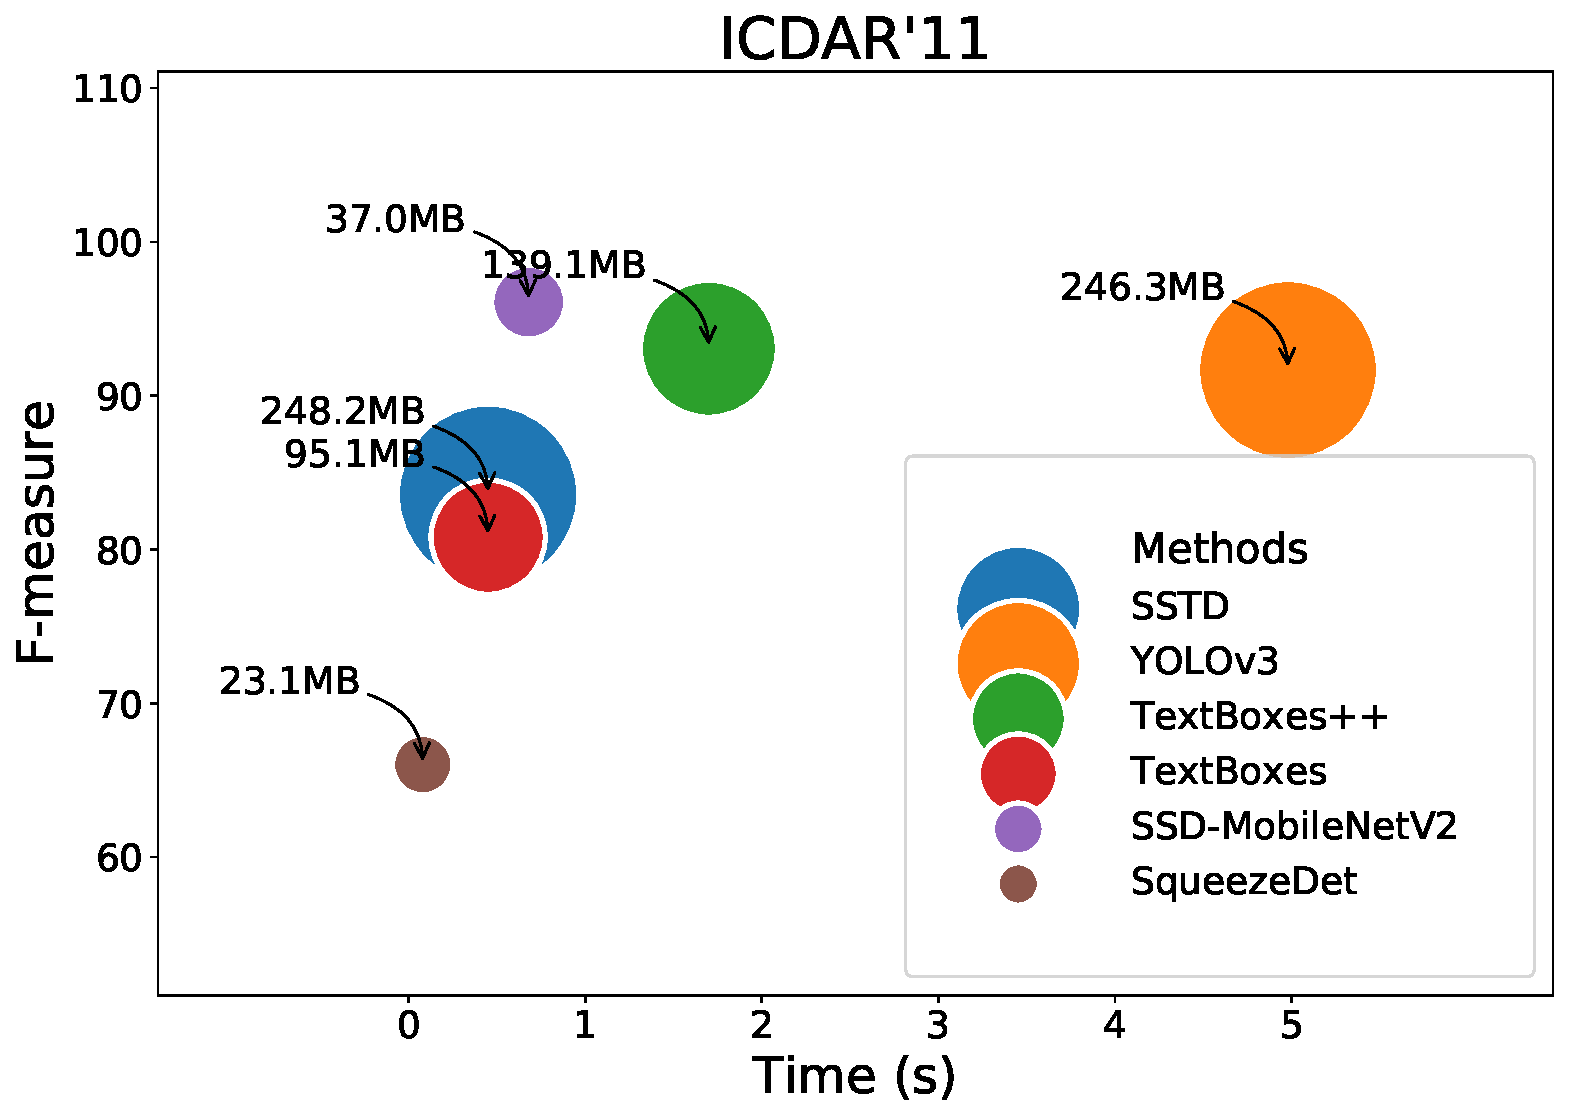
\includegraphics[height=0.25\textheight]{figs/efficacy-and-efficiency/deep-methods-icdar11-f-measure.pdf}
        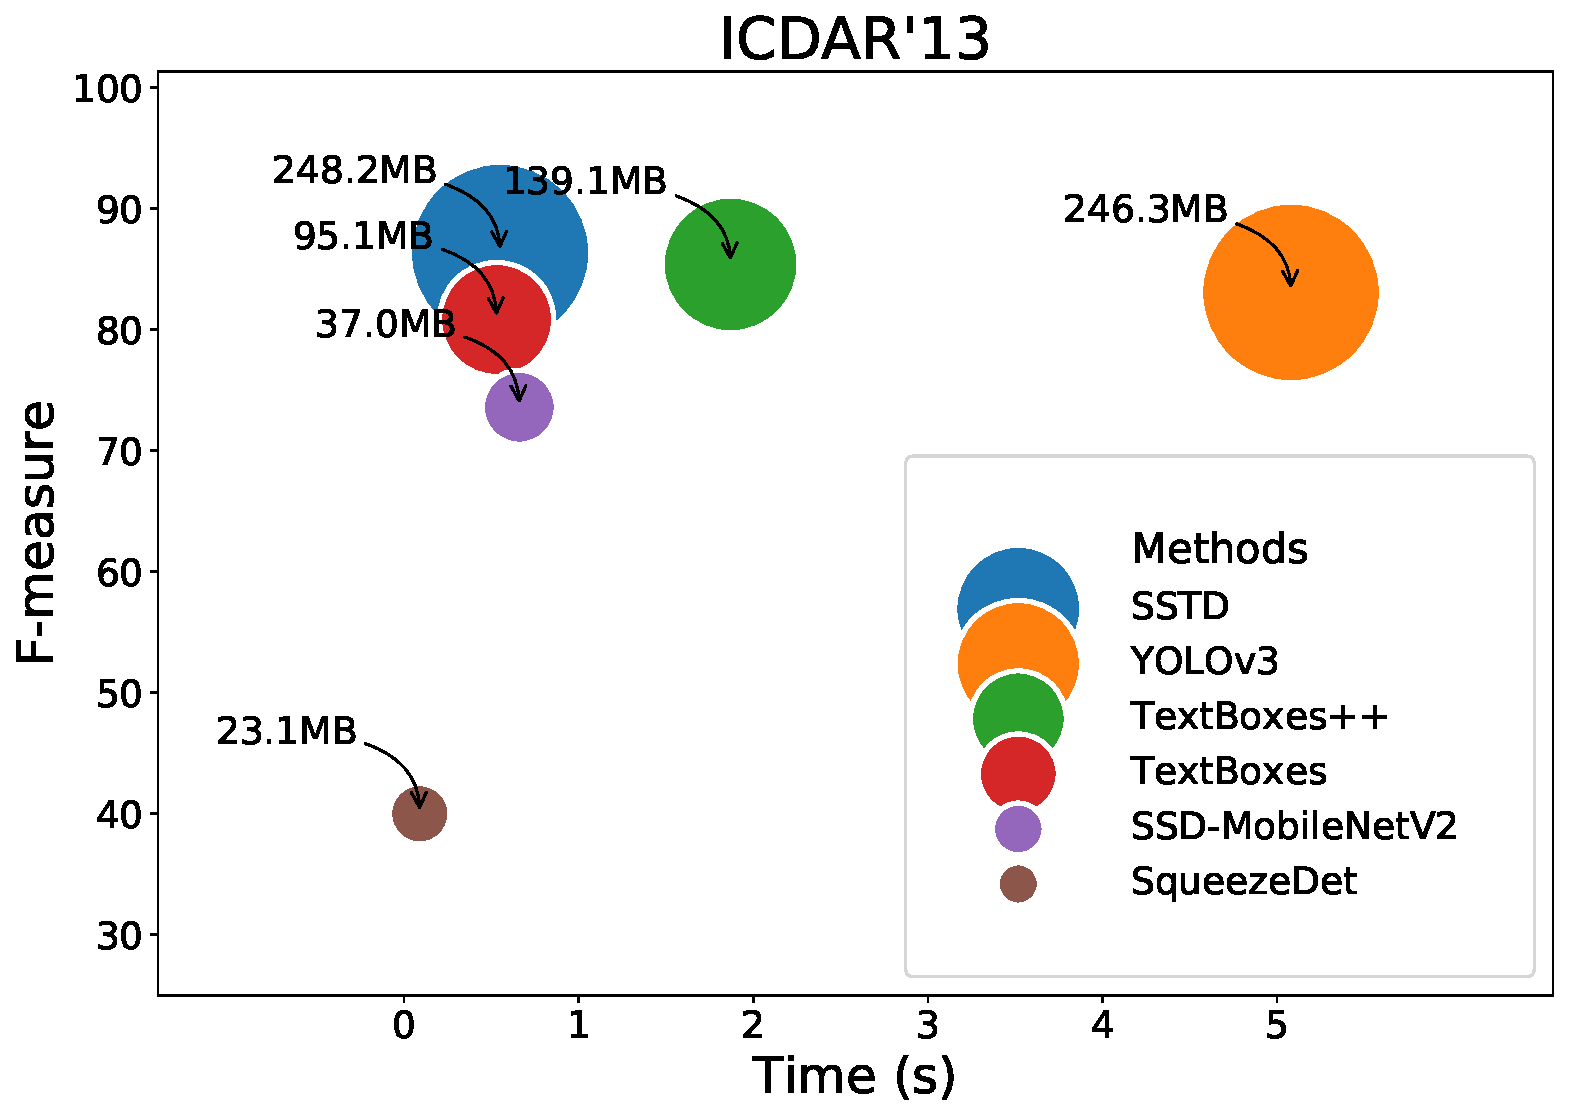
\includegraphics[height=0.25\textheight]{figs/efficacy-and-efficiency/deep-methods-icdar13-f-measure.pdf}
    \end{subfigure}
    \caption{Comparison results among the deep-learning-based methods considering aspects of efficacy and efficiency.}
    \label{fig:deep-methods-efficacy-and-efficiency}
\end{figure}


